\documentclass[../AISTR.tex]{subfiles}
	\ifSubfilesClassLoaded{%
	\bibliography{aistr.bib}%
}{}
\begin{document}

\section{Протоколы взаимодействия вакуумного оборудования}
\subsection{Модель OSI}
Модель \osi{} -- идеальная модель построения сети.

На \refris{fig:osi} показана структура идеальной модели \textit{OSI}. Модель определяет различные уровни взаимодействия систем. Каждый уровень выполняет определённые функции при таком взаимодействии.


\begin{figure}[H]
	\centering
	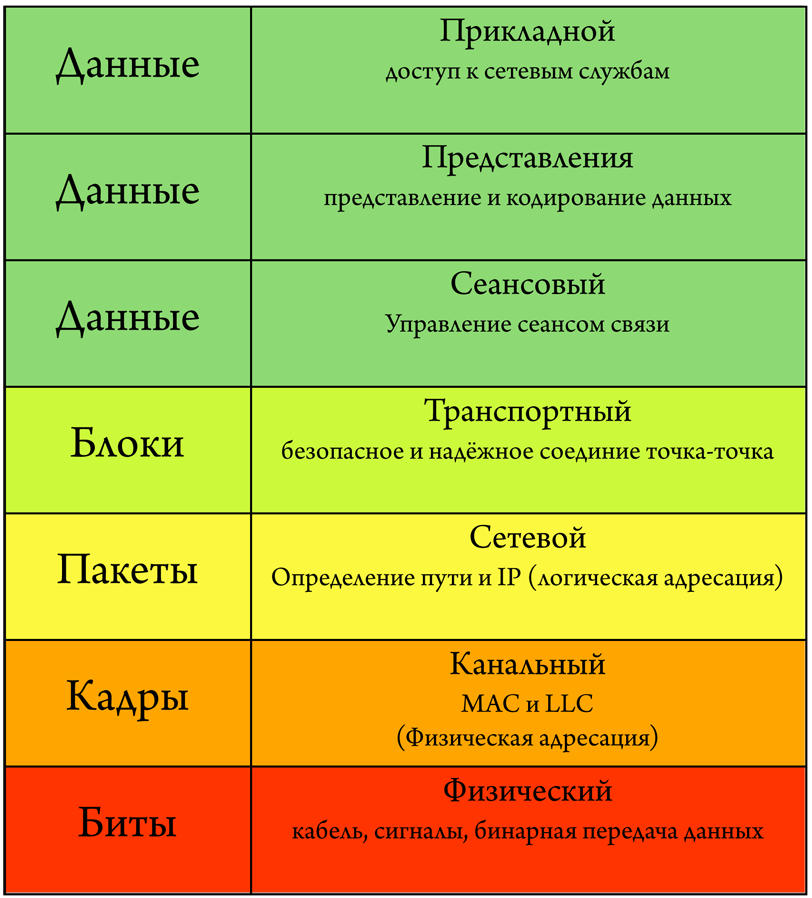
\includegraphics[width=0.6\linewidth]{../images/osi}
	\caption{Уровни модели OSI}
	\label{fig:osi}
\end{figure}

Уровни модели OSI делятся на \cite{kumar_survey_2012} :
\begin{itemize}
	\item \textbf{физический}: предназначен непосредственно для передачи потока данных. Осуществляет передачу электрических или оптических сигналов в кабель или в радиоэфир и, соответственно, их приём и преобразование в биты данных в соответствии с методами кодирования цифровых сигналов;
	\item \textbf{канальный}: предназначен для обеспечения взаимодействия сетей на физическом уровне. Полученные с физического уровня данные проверяет на ошибки, если нужно исправляет, упаковывает во фреймы, проверяет на целостность, и отправляет на сетевой уровень;
	\item \textbf{сетевой}: определяет пути передачи данных. Отвечает за трансляцию логических адресов и имён в физические, за определение кратчайших маршрутов, коммутацию и маршрутизацию, за отслеживание неполадок и заторов в сети;
	\item \textbf{транспортный}: организует доставку данных без ошибок, потерь и дублирования (не все) в той последовательности, как они были переданы. Разделяет данные на фрагменты равной величины, объединяя короткие и разбивая длинные (размер фрагмента зависит от используемого протокола);
	\item \textbf{сеансовый}: управляет созданием/завершением сеанса связи, обменом информацией, синхронизацией задач, определением права на передачу данных и поддержанием сеанса в периоды неактивности приложений. Синхронизация передачи обеспечивается помещением в поток данных контрольных точек, начиная с которых возобновляется процесс при нарушении взаимодействия;
	\item \textbf{представления}: на этом уровне может осуществляться преобразование протоколов и сжатие/распаковка или кодирование/декодирование данных, а также перенаправление запросов другому сетевому ресурсу, если они не могут быть обработаны локально;
	\item \textbf{прикладной}: уровень приложений (англ. Application layer). Обеспечивает взаимодействие сети и приложений пользователя, выходящих за рамки модели OSI. На этом уровне работают изученные в работе протоколы автоматизации промышленных сетей.
\end{itemize}

\subsection{Протокол Modbus}
В настоящее время существует огромное множество промышленных протоколов, используемых в автоматизации. На \refris{fig:divide} показано распределение рынка между протоколами \cite{promwad__2019}:

\begin{figure}[h]
	\centering
	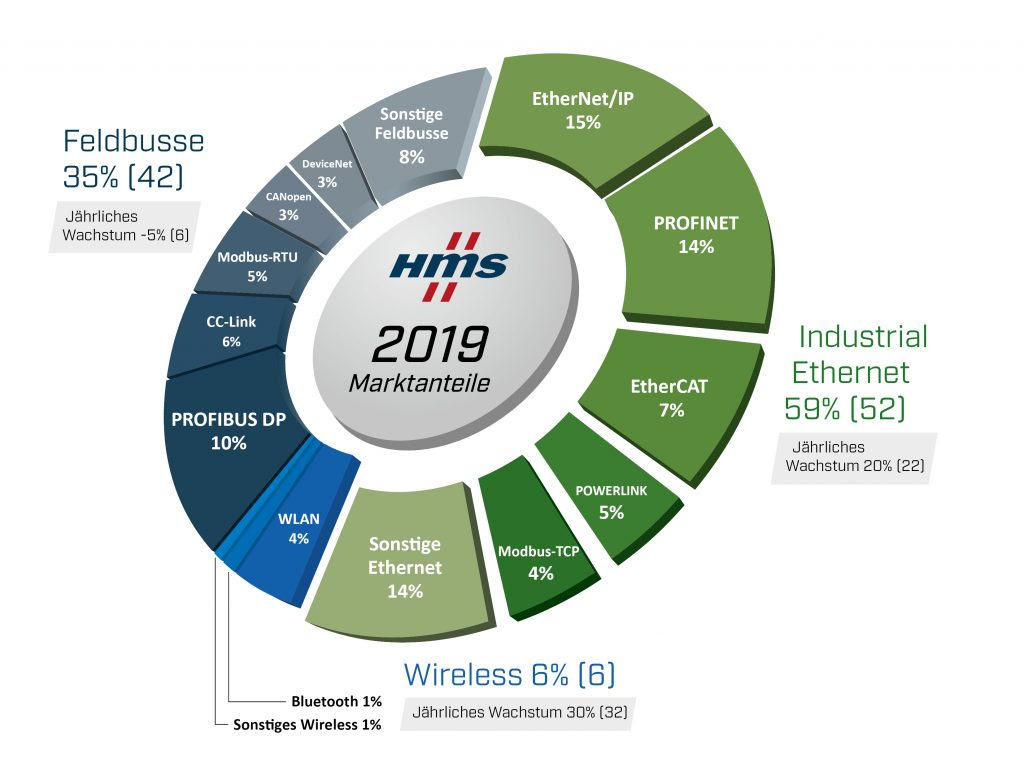
\includegraphics[width=0.8\linewidth]{../images/divide}
	\caption{Диаграмма долей рынка промышленных протоколов}
	\label{fig:divide}
\end{figure}

В России основную долю рынка занимают протоколы \mb и \pb \cite{__2010}, однако \pb уступает своему конкуренту в ряде вещей:
\begin{itemize}
	\item стандарт открыт не полностью;
	\item сложнее в освоении, чем \mb;
	\item в СНГ \mb более популярен.
\end{itemize}

\subsection{Прицип работы протокола Modbus}
\subsubsection{Физический уровень}
Протокол \mb может быть использован со следующими интерфейсами:
\begin{itemize}
	\item \textbf{RS-232/422/485}:  последовательные интерфейсы, широко распространенные в промышленности. Интерфейсы RS-422/485 обеспечивают дальность сигнала до 1200 метров. Используются протоколы \textit{Modbus RTU/ASCII}
	\item \textbf{TCP/IP}: физическим каналом передачи данных могут любые ethernet-ин\-терфейсы. Используется протокол \textit{Modbus TCP}.
\end{itemize}
Существует 3 разновидности протокола \mb{} \cite{_modbus_2021}:
\begin{enumerate}
	\item \mb{} \textit{ASCII}: в котором данные кодируются символами из таблицы ASCII (рис. 1) и передаются в шестнадцатеричном формате и данный формат протокола встречается довольно редко;
	\item \mb{} \textit{RTU}: самый распространенный вариант протокола Modbus, который кодирует данные в двоичном формате и разделяет пакеты с помощью временного интервала;
	\item \mb{} \textit{TCP}:  данные кодируются в двоичном формате и упаковываются в TCP - пакет, для передачи по IP-сетям и предназначен для работы в локальных сетях.
\end{enumerate}

На \refris{fig:modbusphys} показан пример построения схемы контроля за неким объектом при помощи протокола \mb{} \cite{advantech_iot__2019}.

\begin{figure}
	\centering
	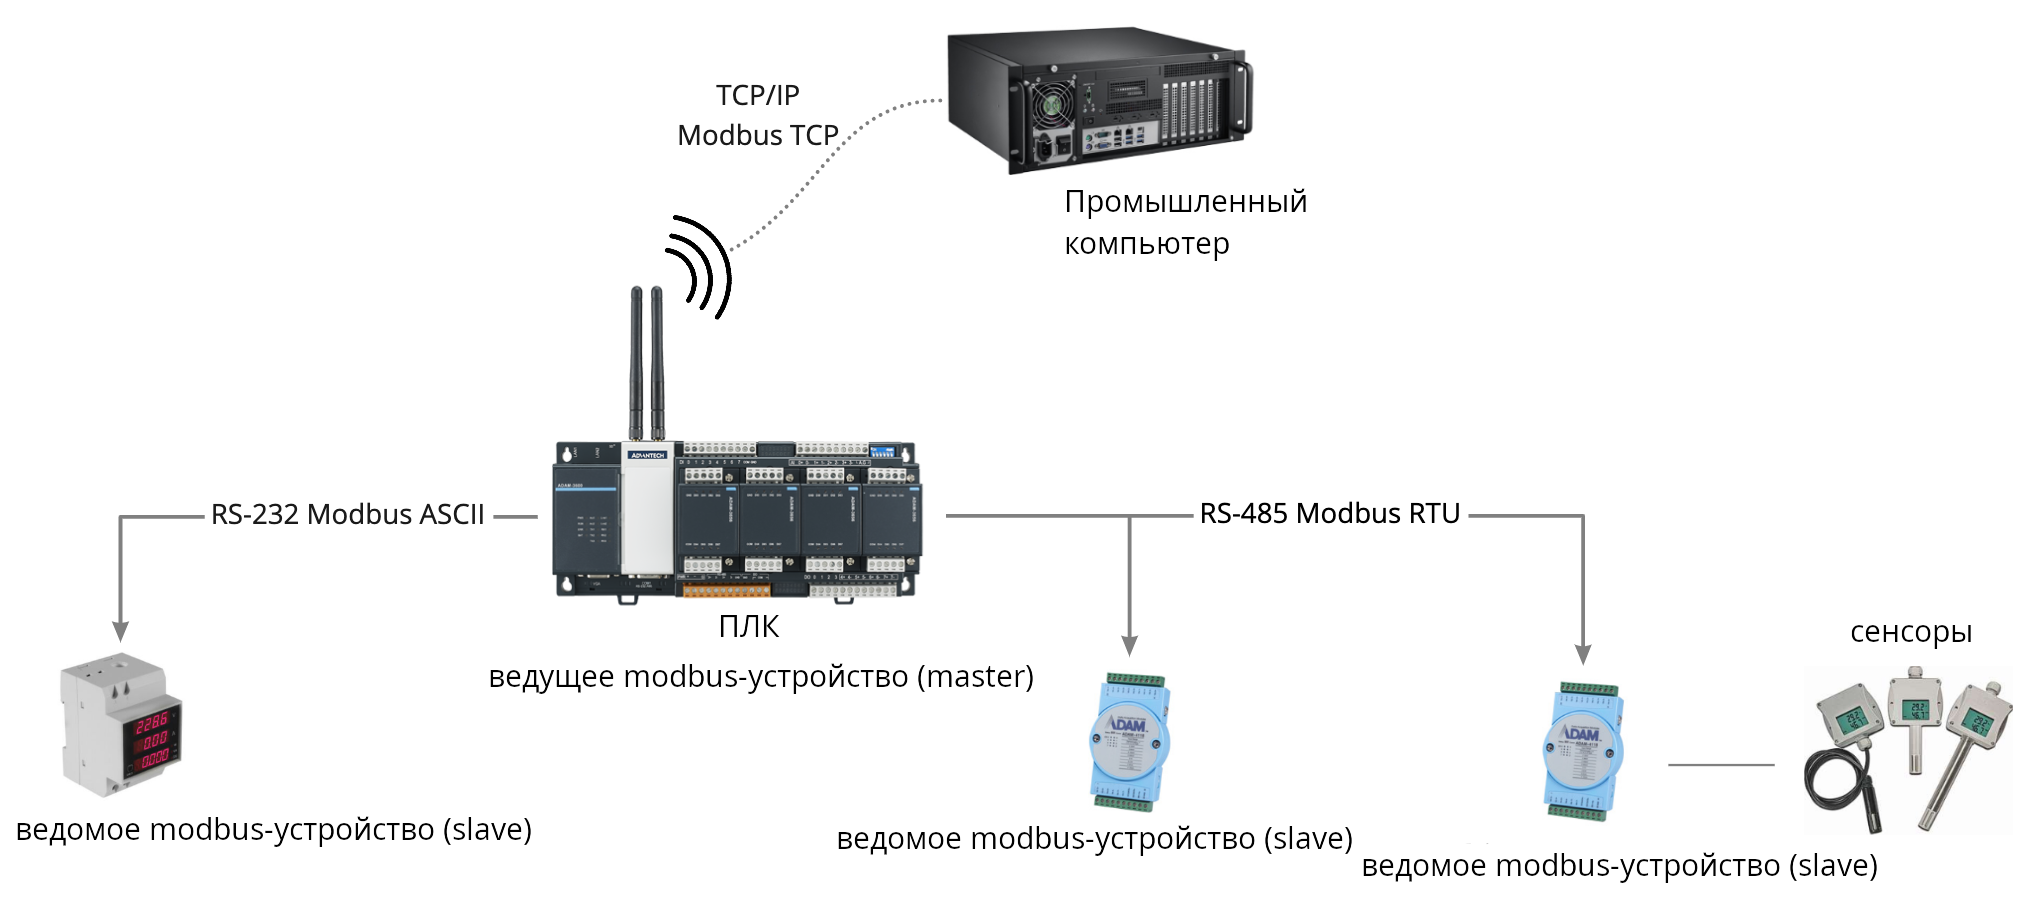
\includegraphics[width=\linewidth]{../images/modbus_phys}
	\caption{Физический уровень протокола \mb{}}
	\label{fig:modbusphys}
\end{figure}
\subsubsection{Логический уровень}
Протокол \mb предполагает одно ведущее устройство и до $247$ ведомых. Обмен данными начинается ведущим устройством. Ведомые не могут начинать передачу и обмениваться данными между собой. В любой момент времени может происходить только один акт обмена. Структуры пакетов \mb при работе 3 способами приведены на \refris{fig:modbusstruct}.
\begin{figure}
	\centering
	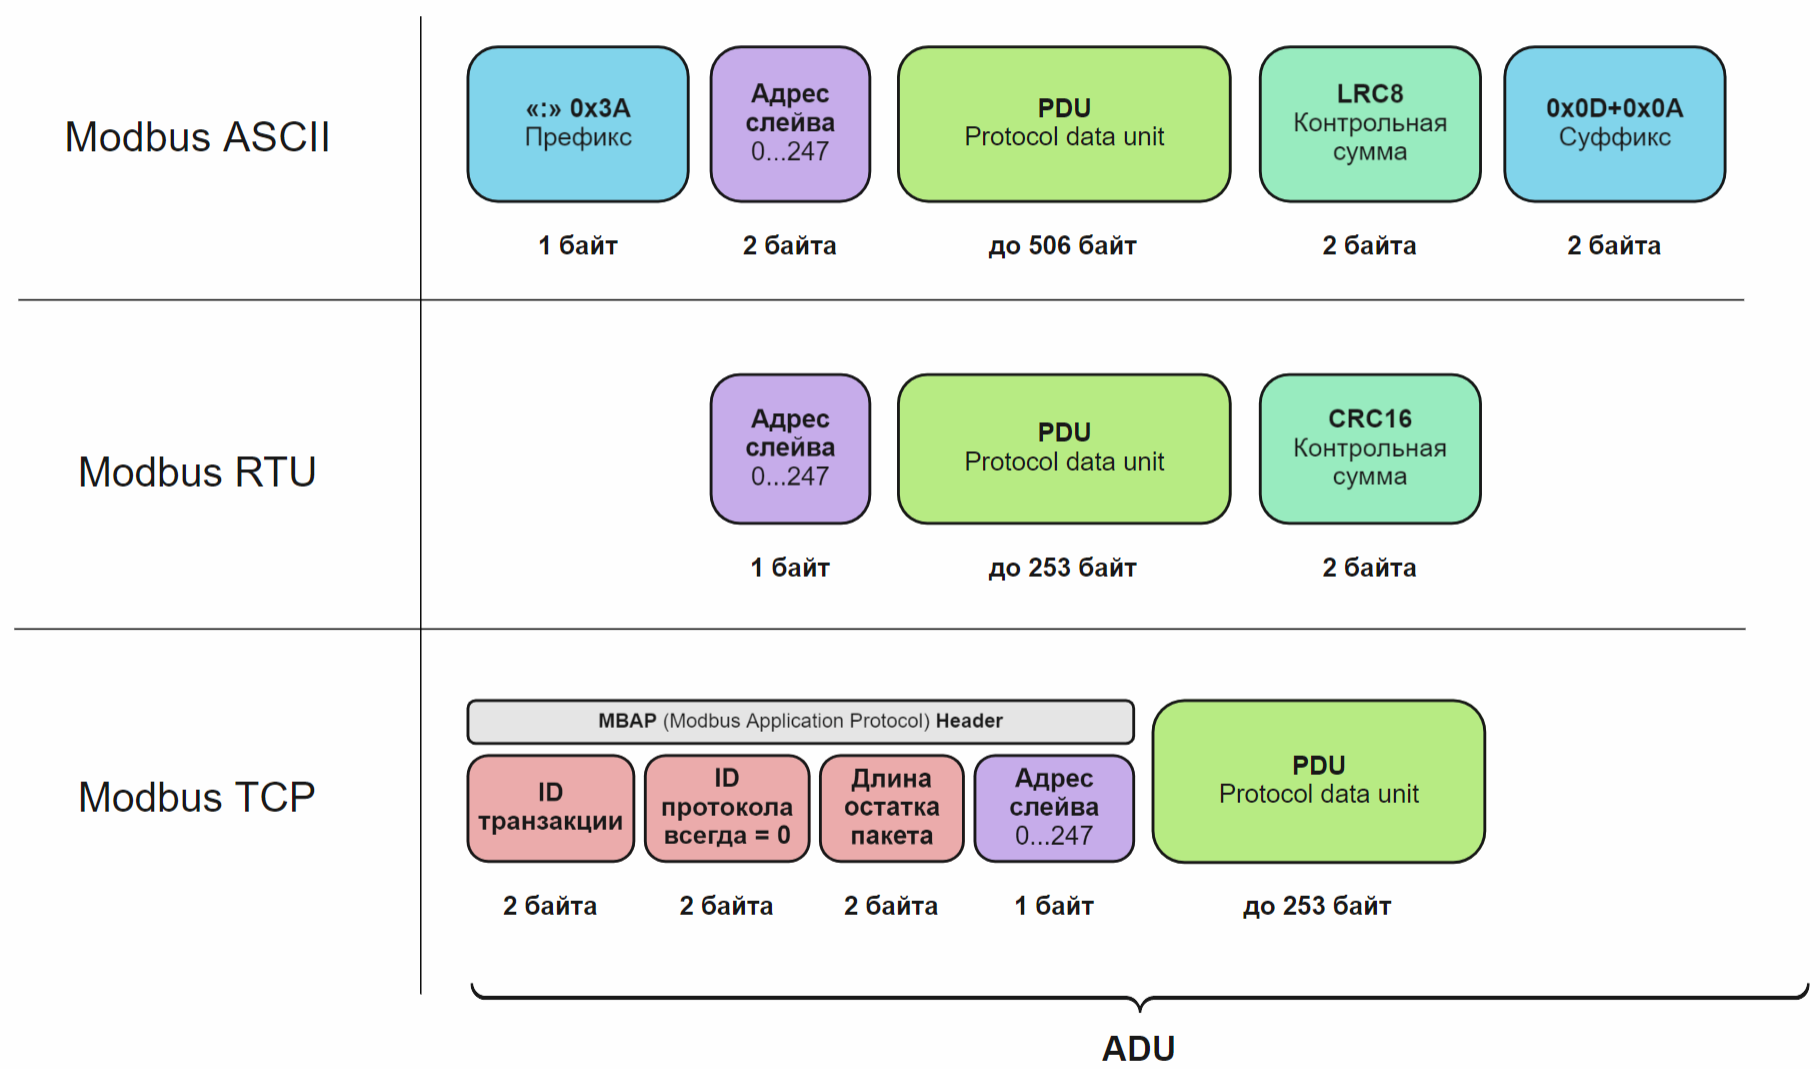
\includegraphics[width=0.9\linewidth]{../images/modbus_struct}
	\caption{Структура пакета \mb}
	\label{fig:modbusstruct}
\end{figure}


\paragraph{Modbus RTU} \label{par:modbusrtu}
Сообщение начинает восприниматься как новое после паузы длиной в $14$ бит. На \refris{fig:modbuspdu} показан формат пакета.
\begin{figure}[h]
	\centering
	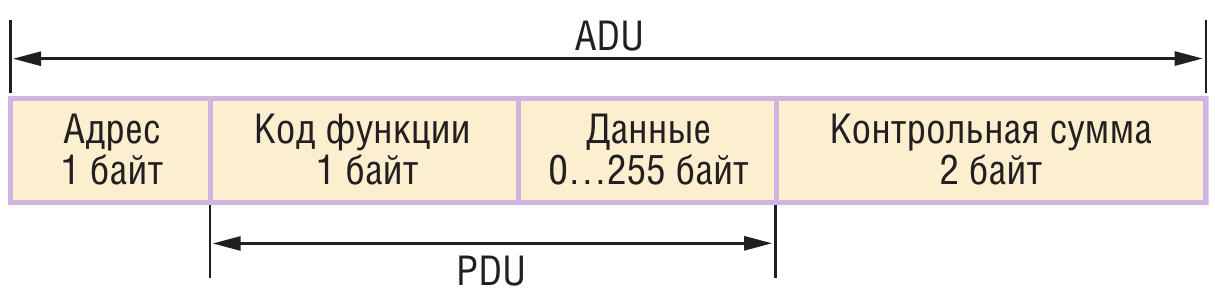
\includegraphics[width=\linewidth]{../images/modbus_PDU}
	\caption{Формат кадра протокола \mb \textit{RTU}}
	\label{fig:modbuspdu}
\end{figure}
У пакета есть следующие поля \cite{__2010}:
\begin{itemize}
	\item \textbf{Адрес:} содержит адрес ведомого устройства. Адрес отправляется даже при ответе на запрос мастера, тем самым всегда понятно откуда пришёл ответ;
	\item \textbf{Код функции:} говорит модулю о том, что ему необходимо сделать;
	\item \textbf{Данные:} тут может содержаться информация о параметрах, которые используются в исполнении команд мастера или показания, передаваемые мастеру;
	\item \textbf{Контрольная сумма:} используется для проверки целостности пакета.
\end{itemize}

\paragraph{Modbus TCP}
Данный протокол используется для того, чтобы подключить устройства, работающие по протоколу \mb к сети \textit{Internet} \cite{__2018-1}. То есть, в соответствии со стандартом \osi (см. \refris{fig:osi}) на транспортном уровне используется протокол \tcp, а на прикладном -- \mb. В этом случае проверка целостности пакета ложится на протокол \tcp. Структура протокола \mb \tcp приведена на \refris{fig:modbustcp}. 
\begin{figure}[h]
	\centering
	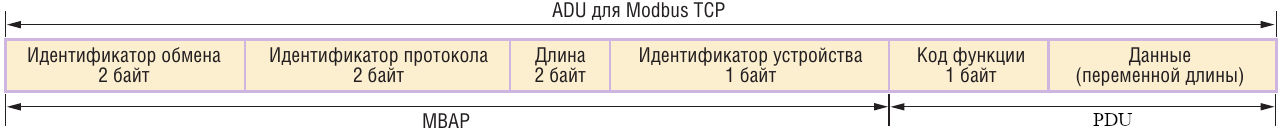
\includegraphics[width=1\linewidth]{images/modbus_TCP}
	\caption{Формат кадра протокола \mb \tcp}
	\label{fig:modbustcp}
\end{figure}
У пакета есть следующие поля \cite{__2010}:
\begin{itemize}
	\item \textbf{Идентификатор обмена:} используется для идентификации сообщения в случае,	когда в пределах одного TCP - соединения клиент посылает серверу несколько сообщений без ожидания ответа после каждого сообщения;
	\item \textbf{Идентификатор протокола:} всегда выставлен на 0 (как и протокола \tcp);
	\item \textbf{Длина:} указывает количество следующих байтов;
	\item \textbf{Идентификатор устройства:} адрес slave - устройства;
	\item \textbf{Код функции:} аналогично \refpar{par:modbusrtu};
	\item \textbf{Данные:} аналогично \refpar{par:modbusrtu}.
\end{itemize}

\begin{figure}[h]
	\centering
	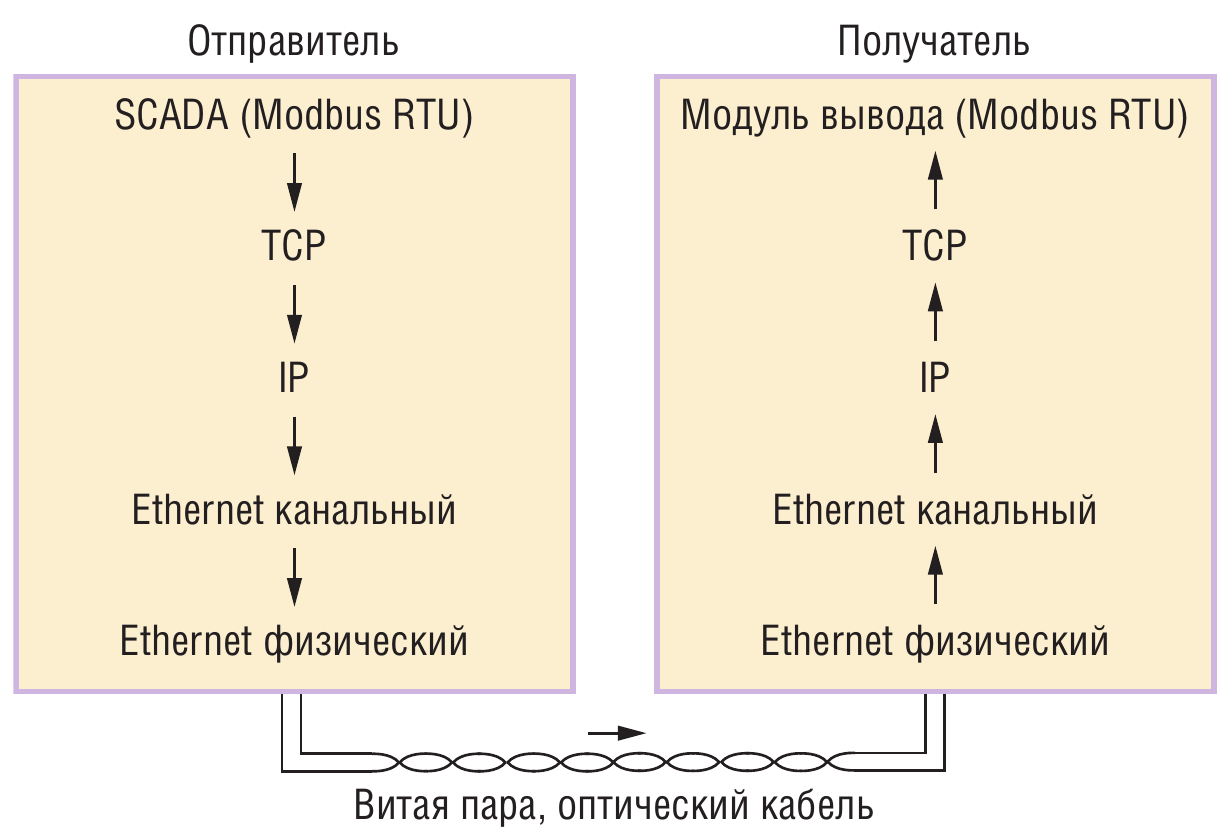
\includegraphics[width=0.7\linewidth]{images/modbus_tcp}
	\caption{Процесс передачи пакетов \mb \textit{RTU} по сети \tcp}
	\label{fig:modbustcp_ip}
\end{figure}

Как можно заметить, \mb \textit{RTU}, оказывается ``вшит'' в пакет \tcp, тем самым получается \mb \tcp. На \refris{fig:modbustcp_ip} показан принцип работы такой системы \cite{__2010}:
\begin{itemize}
	\item коды функций передаются с прикладного уровня на транспортный (\mb -- \tcp), добавление заголовка \tcp;
	\item передача на сетевой уровень, добавление блока \textit{IP};
	\item передача на канальный уровень, а затем на физический (\textit{Ethernet})
\end{itemize}
После прохождения через канал связи пакет начинает обратное движение согласно модели \osi (см. \refris{fig:osi}). 



Более подробно о работе с протоколом \mb{} можно узнать в документации \cite{swales_open_1999}.
\end{document}